\section{Results}\label{sec:results}

\subsection{Model Comparison}

Table~\ref{tab:model_comparison} reports test-set performance for all configurations, sorted by RMSE.

\begin{table}[H]
\centering
\caption{Model comparison on the test set (213 samples), sorted by RMSE. Best values in \textbf{bold}.}
\label{tab:model_comparison}
\begin{tabular}{@{}lrrrrrr@{}}
\toprule
\textbf{Model} & \textbf{MAE} & \textbf{RMSE} & \textbf{$R^2$} & \textbf{MAPE (\%)} & \textbf{RAE} & \textbf{WI} \\
\midrule
CatBoost-PPSO & \textbf{1{,}496.2} & \textbf{1{,}895.5} & \textbf{0.9135} & \textbf{0.89} & \textbf{0.280} & \textbf{0.9774} \\
CatBoost & 1{,}679.4 & 2{,}118.8 & 0.8919 & 0.99 & 0.314 & 0.9709 \\
Linear Reg. & 1{,}693.4 & 2{,}119.2 & 0.8919 & 1.01 & 0.317 & 0.9731 \\
XGB-PPSO & 1{,}687.8 & 2{,}165.6 & 0.8871 & 1.00 & 0.315 & 0.9697 \\
Random Forest & 1{,}774.0 & 2{,}237.6 & 0.8795 & 1.05 & 0.332 & 0.9653 \\
RF-PPSO & 1{,}794.1 & 2{,}283.9 & 0.8744 & 1.06 & 0.335 & 0.9634 \\
XGBoost & 1{,}833.4 & 2{,}313.4 & 0.8712 & 1.08 & 0.343 & 0.9652 \\
\bottomrule
\end{tabular}
\end{table}

Key observations:

\begin{enumerate}
    \item \textbf{CatBoost-PPSO leads on all six metrics}: $R^2 = 0.914$ (over 91\% of demand variance explained), RMSE of 1{,}895.5\,MWh ($\approx$1.1\% of mean daily demand), MAPE of 0.89\%.
    \item \textbf{PPSO benefits are model-dependent.} PPSO improves CatBoost (RMSE $-$10.5\%) and XGBoost ($-$6.4\%), but slightly degrades Random Forest ($+$2.1\%), indicating mild overfitting of the cross-validated fitness to the training period. Because all models received the same budget, these deltas make clear that CatBoost-PPSO's lead is not an artefact of preferential tuning.
    \item \textbf{Linear Regression is competitive}, tied with default CatBoost on RMSE---evidence that the engineered autoregressive features (lag-1, rolling means) render much of the problem linear.
    \item \textbf{All models exceed $R^2 = 0.87$ and WI $= 0.96$}, confirming the 16-feature set captures the dominant demand drivers.
\end{enumerate}

\subsection{Prediction Behaviour}

Figure~\ref{fig:predictions} shows actual versus predicted demand for CatBoost-PPSO over the 213-day test period. The model reproduces weekly cyclicity (weekend dips), tracks demand level shifts, and errs most on extreme holiday-related drops.

\begin{figure}[H]
    \centering
    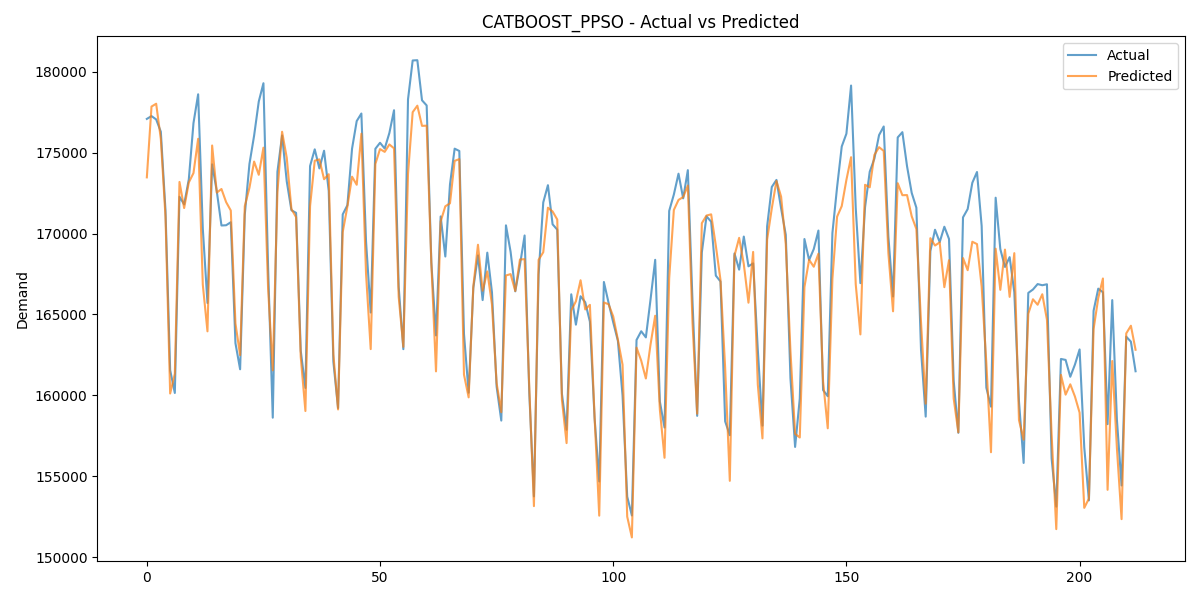
\includegraphics[width=0.88\textwidth]{eval/images/predictions_catboost_ppso.png}
    \caption{Actual vs.\ predicted daily electricity demand (MWh), CatBoost-PPSO, test set.}
    \label{fig:predictions}
\end{figure}

\subsection{Feature Importance}

Figure~\ref{fig:feature_importance} presents CatBoost-PPSO importance scores. Autoregressive features dominate (\texttt{demand\_lag\_1}, rolling means), followed by \texttt{day\_of\_week}; weather variables (temperature, humidity, CCI) contribute meaningful mid-rank exogenous signal. The same hierarchy appears across RF and XGBoost, confirming robustness.

\begin{figure}[H]
    \centering
    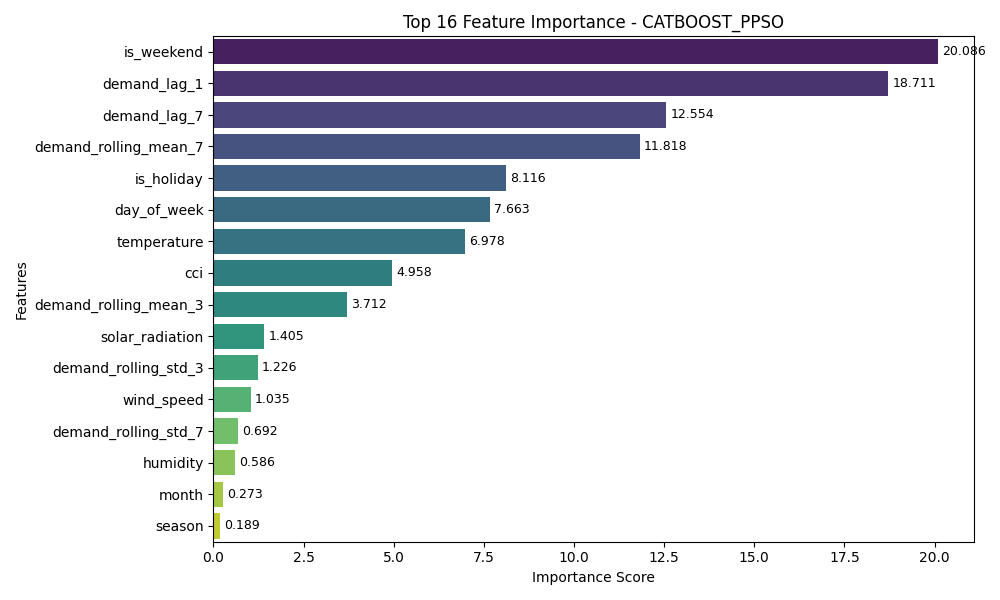
\includegraphics[width=0.78\textwidth]{eval/images/feature_importance_catboost_ppso.png}
    \caption{Feature importance, CatBoost-PPSO. Autoregressive features dominate, with weather variables providing secondary signal.}
    \label{fig:feature_importance}
\end{figure}

\subsection{Impact of PPSO Optimisation}

Table~\ref{tab:ppso_impact} quantifies the tuning effect on CatBoost, the model with the largest gain.

\begin{table}[H]
\centering
\caption{Impact of PPSO hyperparameter optimisation on CatBoost.}
\label{tab:ppso_impact}
\begin{tabular}{@{}lrrr@{}}
\toprule
\textbf{Metric} & \textbf{CatBoost (default)} & \textbf{CatBoost-PPSO} & \textbf{Improvement} \\
\midrule
MAE (MWh) & 1{,}679.4 & 1{,}496.2 & $-$10.9\% \\
RMSE (MWh) & 2{,}118.8 & 1{,}895.5 & $-$10.5\% \\
$R^2$ & 0.8919 & 0.9135 & $+$2.2 pp \\
MAPE (\%) & 0.99 & 0.89 & $-$10.6\% \\
RAE & 0.314 & 0.280 & $-$10.9\% \\
WI & 0.971 & 0.977 & $+$0.6 pp \\
\bottomrule
\end{tabular}
\end{table}

Compared with the reference study \parencite{zhang2023catboostppso} ($R^2 = 0.971$ on hourly single-customer data), the lower $R^2$ here (0.914) is expected: daily national demand aggregates heterogeneous consumption across millions of consumers, adding unexplained variance. The methodology nonetheless transfers effectively across scale, resolution, and climate.
